%\thispagestyle{empty}
\newgeometry{top=4cm, bottom=4cm, left=4cm, right=4cm} 

\setlength{\parindent}{2em}
\setlength{\parskip}{0em}
\setlength{\columnsep}{2em}

\begin{figure}
    \centering
    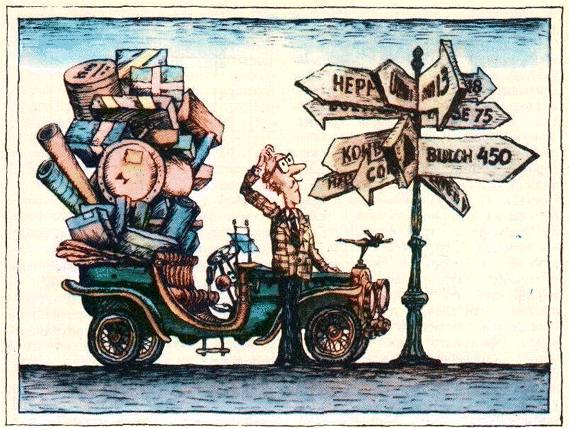
\includegraphics[width=\columnwidth]{pic2.png}
\end{figure}

\begin{multicols}{2}

\noindent
\textit{Е. Габович} \\

\noindent
\huge
\textbf{Задача \\коммивояжера}\\

\footnotesize
\noindent
\textbf{<<Пользуйтесь услугами Аэрофлота!>>}

\normalsize
\noindent
Два автомобилиста, инженер А. Невский и экономист Б. Литейный, решили съездить в Закавказье, посетить Баку и Тбилиси, заехать в Москву, Киев и Горький, а затем вернуться в родной Ленинград. Начали обсуждать маршрут путешествия. Невский посмотрел на карту и предложил такую последовательность посещения городов:

\textit{Л $\rightarrow$ М $\rightarrow$ Г $\rightarrow$ Б $\rightarrow$ Т $\rightarrow$ К $\rightarrow$ Л}

\noindent
Литейный же. достав атлас автомобильных дорог, выписал расстояния между нужными им городами в табличку (см. таблицу 1) и подсчитал 

\vfill\null
\columnbreak

\noindent
длину предложенного маршрута: $696+410+2937+579+1863+1207= \linebreak
=7692$ км. <<Длинновато! - сказал \linebreak
он. - Расстояние аэрофлотское! А нельзя ли короче? Уверен ли ты, что этот маршрут является кратчайшим?>>

Уверенности такой у Невского не было. Более того, объяснить, почему он решил ехать именно так, Невский не мог. Просто интуиция подсказывала ему, что такой маршрут, если и

\begin{flushright}
\footnotesize
    Т а б л и ц а 1
\end{flushright}

\noindent
\resizebox{\columnwidth}{!}{
\textit{
\begin{tabular}{|c|c|c|c|c|c|c|}
    \hline
    %Город & Л & М & К & Б & Т & Г \\
    Город & Л & М & К & Б & Т & Г \\
    \hline
    Ленинград & - & 696 & 1207 & 3223 & 2797 & 1106 \\
    Москва & 696 & - & 858 & 2527 & 2101 & 410 \\
    Киев & 1207 & 858 & - & 2283 & 1863 & 1268 \\
    Баку & 3223 & 2527 & 2283 & - & 579 & 2937 \\
    Тбилиси & 2797 & 2101 & 1863 & 579 & - & 2511 \\
    Горький & 1106 & 410 & 1286 & 2937 & 2511 & - \\
    \hline
\end{tabular}}}

\begin{flushright}
    \vfill\null
    \textbf{11}
\end{flushright}

\end{multicols}